%!TEX root = Constructive Alignment for Introductory Programming.tex

\chapter{Evaluation of Teaching and Learning Context} % (fold)
\label{cha:evaluation}

\graphicspath{{Figures/Evaluation/}}

\section{Research Design} % (fold)
\label{sec:research_design}

\subsection{Action Research} % (fold)
\label{sub:action_research}

Due to the practical nature of this research, its focus on student learning, and the embedded reflective process it was decided to follow a Practical Action Research \cite{Creswell:2008} design based on Mills' \cite{Mills:2010} \emph{dialectic action research spiral}. This model, shown in \fref{fig:mills_spiral}, includes a four step process: (1) identify an area of focus, (2) collect data, (3) analyse and interpret the data, and (4) develop an Action Plan. %The Iterations section documents the \emph{focus}, \emph{plan}, \emph{data}, and \emph{analysis and reflections} per iteration.

\begin{figure}[htbp]
  \centering
  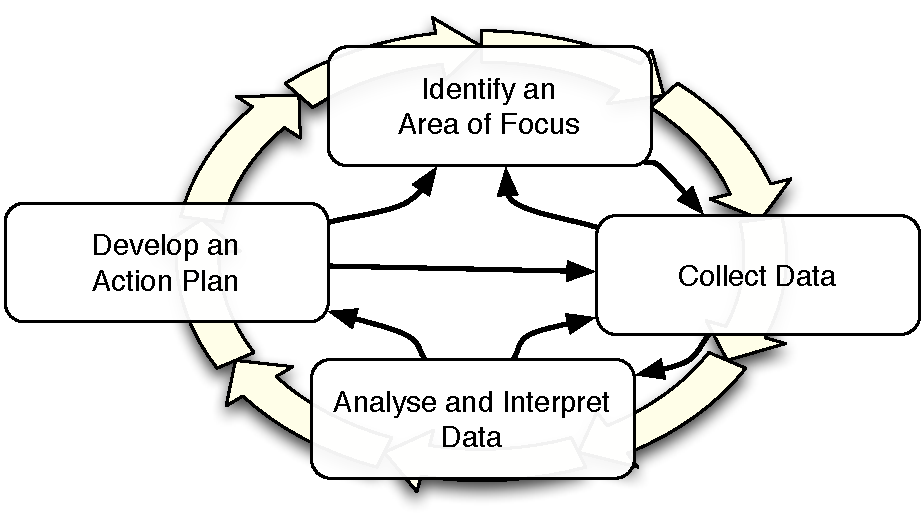
\includegraphics[width=0.7\columnwidth]{MillsSpiral}
  \caption{Mills \cite{Mills:2010} Dialectic Action Research Spiral.}
  \label{fig:mills_spiral}
\end{figure}

Iterations in this action research project aligned to teaching periods that included the delivery of one, or more, of the programming units discussed in \cref{cha:example_impl}. Each iteration included an \emph{action plan} related to implementing the approach from \cref{cha:approach}, which influenced the \emph{focus} for the iteration, the data collected, and the analysis performed.

The overall focus for this research was on the development, application and iterative improvement of the model from \cref{cha:approach}. The iterative nature of the action research process meant that the specific focus in each teaching period addressed relevant aspects of the model, based on its current state and feedback from previous iterations. 

Data collection included analysis of student portfolios, student grades, unit documentation and staff reflections, as illustrated in \fref{fig:research_data}. Each of these is described in the following paragraphs, with the ethical considerations related to using student work being discussed in \sref{sub:addressing_ethical_concerns}.

\begin{figure}[thb]
  \centering
  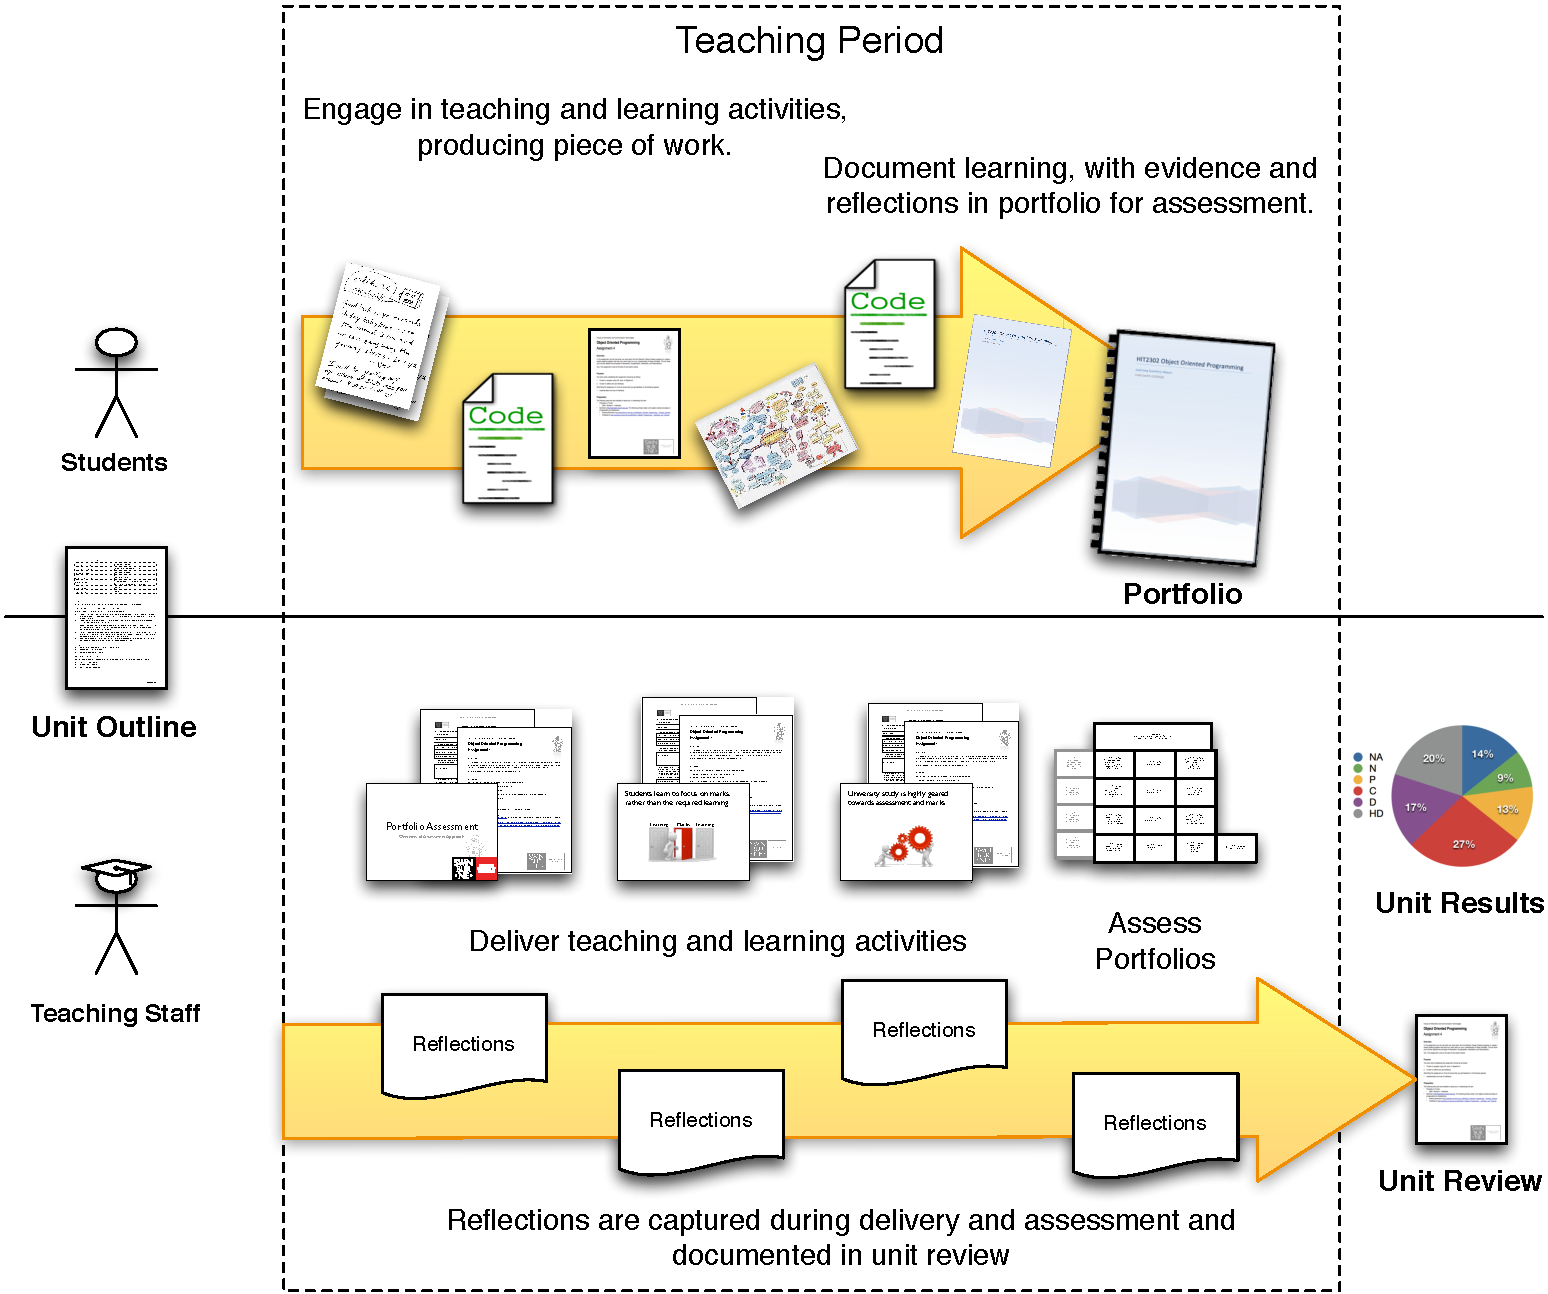
\includegraphics[width=\textwidth]{ResearchData}
  \caption{Illustration of the various documents used in the data collection for this research.}
  \label{fig:research_data}
\end{figure}

Thematic analysis was used to examine reflections in student portfolios, which is discussed further in \sref{sub:thematic_analysis}. As the thematic analysis of student portfolios was time consuming, it was not performed in all iterations. In teaching periods where a thematic analysis of the portfolios was not performed, the student grades and staff reflections provide insights into the composition of student portfolios.

Unit documentation included the Unit Outline and Unit Review documents. The Unit Outline included the intended learning outcomes and assessment criteria used in the given teaching period. This document was provided to students prior to the commencement of the teaching period and was an actively used document by both teaching staff and students. The Unit Review document was created after results were reported, and captured details of student perceptions of the teaching, teaching and learning approach, results, unit management, and any planned changes for future delivery of the unit. These documents were prepared by the Unit Panel, which included input from all teaching staff.

% The learning environment has been found to influence students' approach to learning \cite{Entwistle:1990,Entwistle:1991,Kember:2007}, and perceptions of these environments have been shown to directly, and indirectly, influence learning outcomes \cite{Meyer:1990,Lizzio:2002}. This research attempts to capture this using results from the University's student satisfaction surveys.

Staff reflections indicated the qualities exhibited in the student portfolios for a given semester. Staff reflections were captured both during the semester and after the portfolios were assessed. These reflections were recorded in notes, which in many cases were then summarised in the Unit Review document.

Student grades provide an indication of how well students performed in the given semester. Together with the staff reflections, these results provide insight into the learning outcomes students achieved - insights not available by considering students grades alone.

% subsection action_research (end)

\subsection{Thematic Analysis of Reflections} % (fold)
\label{sub:thematic_analysis}

Reflections in student portfolios provide a wealth of information. To help identify themes and patterns in the portfolios it was decided to perform a thematic analysis using the process outlined by \citet{Braun:2008}. This process involves six phases (with some terminology adapted for clarity):
\begin{enumerate}[noitemsep,nolistsep]
  \item Familiarising yourself with the data
  \item Generating initial themes,
  \item Searching for strong themes
  \item Reviewing themes
  \item Defining and naming themes
  \item Producing the report
\end{enumerate}

In each teaching period where a thematic analysis was performed, familiarity with the data was obtained early in the process with all portfolios being read as part of the unit assessment. At the end of the unit assessment, teaching staff made notes related to general issues, progress, and the overall quality of portfolios. This was part of standard unit delivery procedures, with the resulting reflections being summarised in the Unit Review document as mentioned in \sref{sub:action_research}.

Once the portfolios were made available for this research initial themes were generated by revisiting the reflective component of each portfolio and looking for the qualities under examination. These themes were then documented, and recorded in a spreadsheet. The spreadsheet software was used to collate the themes and record the portfolio details of where these issues had been mentioned, along with any illustrative comments using the students own words.

In phases 3 through 5 the identified themes were broadly grouped together, and then each broad group was examined for sub-themes. All of the themes identified in the examination of student portfolios were maintained in the final categorised results. Themes that did not clearly relate to any of the identified groups were grouped together as a miscellaneous group.

In the reporting of this analysis we present the raw results, grouped into the identified themes. Illustrative quotes from the student reflections are provided to help define the themes.

% subsection thematic_analysis_of_reflections (end)


\subsection{Addressing Ethical Concerns} % (fold)
\label{sub:addressing_ethical_concerns}

Participants in this study were students of the investigators, and so it was important to design an appropriate process whereby students could offer informed consent to participate in the research with no risk of coercion. The student-teacher relationship was the main source of potential ethical problems for this research, with perceptions of coercion being the central concern. 

This issue is further complicated by the fact that the researchers may teach both the first and second programming units, for example students may undertake the introductory programming unit in the first half of the year, and the object oriented programming unit in the second half of the year. As most students who complete the first unit progressed to the second unit the following semester, there was the potential for the perception of coercion in this second unit.

An appropriate research protocol was developed, and given ethical approval from Swinburne's Human Research Ethics Committee. \fref{fig:ethics_process} shows an overview of this process. 

\begin{figure}[thb]
  \centering
  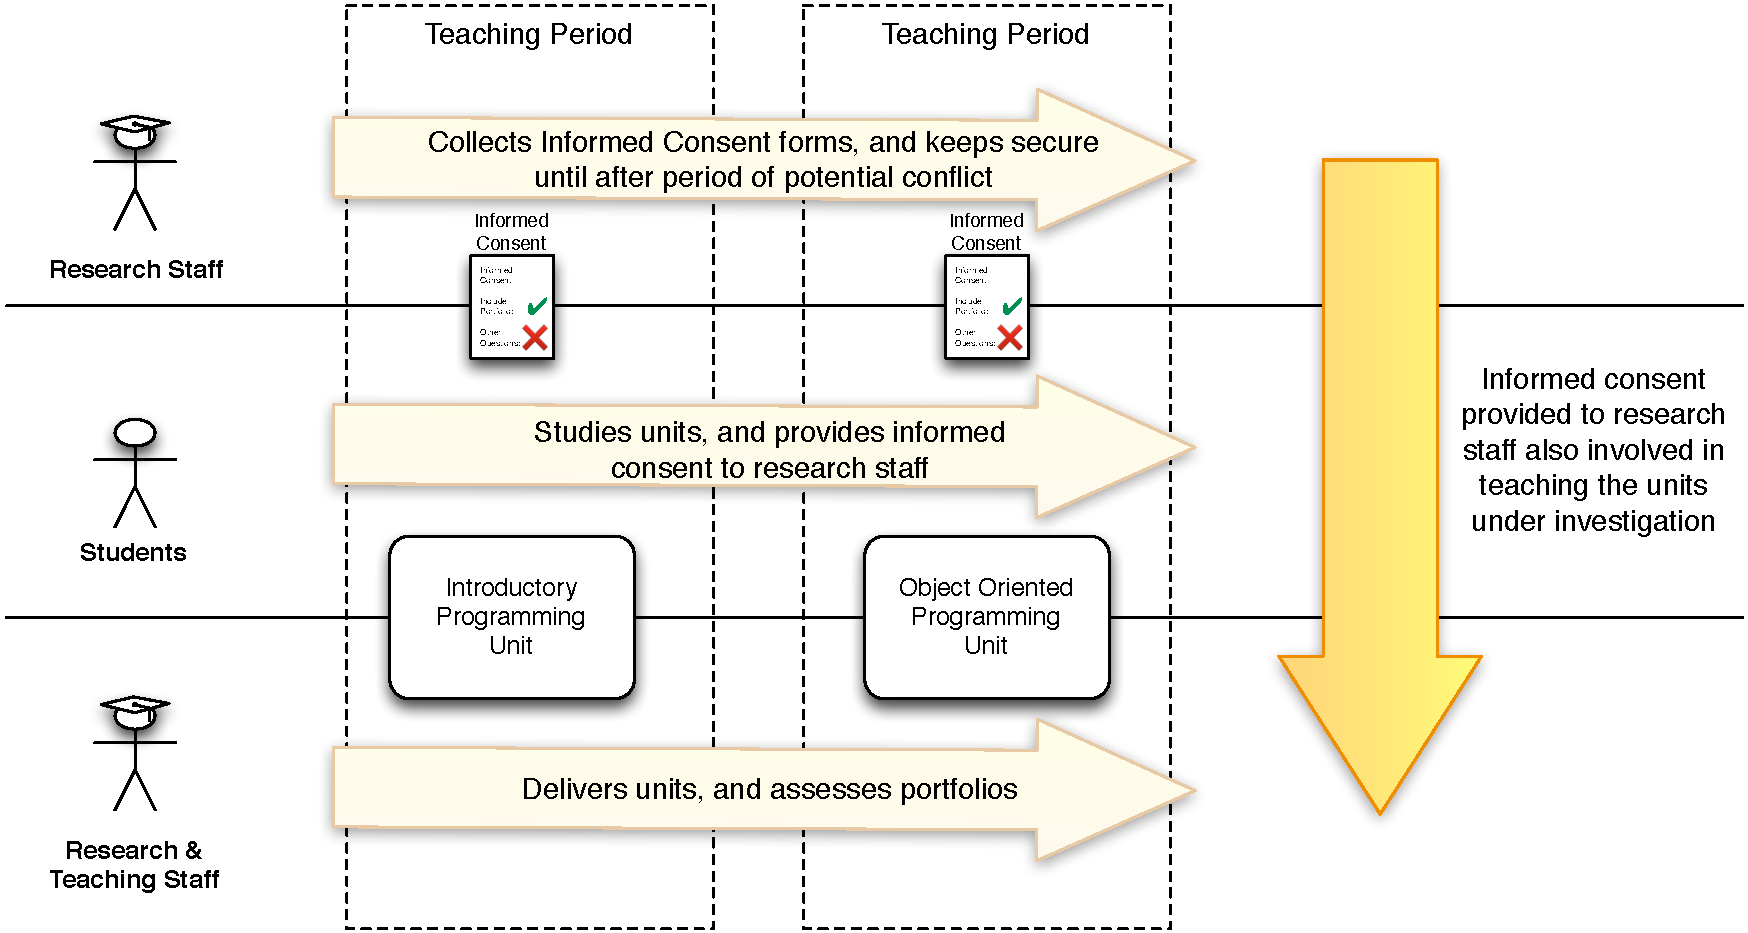
\includegraphics[width=\textwidth]{EthicsProcess}
  \caption{Overview of the process to avoid perceptions of coercion. Informed Consent forms were completed by students in both the introductory programming and object oriented programming units. These forms are collected by researchers not directly involved in the teaching of the unit. The informed consent forms are only made available to the staff involved in teaching the unit after the both units are complete.}
  \label{fig:ethics_process}
\end{figure}

Printed Informed Consent forms were distributed to students in lectures during the teaching period. The forms were completed by all students, and indicated their willingness to have their work included in the research. Students were informed that participation in the research was voluntary, and their response would in no way influence their results or relationship with the university.

To avoid any perception that student responses could in any way affect their results, the Informed Consent forms were withheld from researchers involved in teaching these students until the period of potential influence was deemed to have passed. Until such time, the forms were kept in a sealed envelope in a locked cabinet at Swinburne by the researchers who were not directly involved in teaching of the units. Additionally, all students were required to complete and sign the forms, indicating if they wished to participate or not. In this way it was not be possible to determine those who did, or did not, wish to participate simply by observing those who sign the form.

% \begin{itemize}[noitemsep,nolistsep]
	% \item The Unit Summary Survey was voluntary and anonymous. No identifying information was collected within the questionnaire and there was no means of matching responses with individual students.
	% \item The informed consent forms that indicated if students were willing to have their responses to the Initial Survey and their Portfolio work (for the thematic analysis) included in this research were withheld from researchers involved in teaching these students until the period of potential conflict was deemed to have passed. Until such time, the forms were kept in a sealed envelope in a locked cabinet at Swinburne by the researchers who were not directly involved in teaching of the units. 
	% \item The informed consent forms that indicated if students were willing to have their Portfolio work included in this research (for the thematic analysis) were withheld from researchers involved in teaching these students until the period of potential conflict was deemed to have passed. Until such time, the forms were kept in a sealed envelope in a locked cabinet at Swinburne by the researchers who were not directly involved in teaching of the units. 
	% \item Additionally, all students were required to complete and sign the forms, indicating if they wished to participate or not. In this way it was not be possible to determine those who did, or did not, wish to participate simply by observing those who sign the form.
	% \item The Focus Group will be organised and run by researchers not involved in the teaching and assessment of the unit. Data from the Focus Groups will be transcribed into an encoded form using an encoding scheme whereby the student names and ids will not be known by researchers involved in teaching the units until after the period of potential conflict is deemed to have passed. After this period has passed the same encoding scheme will be used to encode responses to the Initial Survey, Progress Surveys, and data collected from the Thematic Analysis.
% \end{itemize}

The period of potential influence was deemed to have passed based on the following:
\begin{itemize}[noitemsep,nolistsep]
	\item For the introductory programming units where the researchers were not involved in teaching a follow on unit, the period of potential influence was deemed to have passed once the results for the introductory programming unit were published.
	\item For the introductory programming units where the researchers were involved in the teaching the follow on unit, the period of potential influence was deemed to have passed once the results for the \emph{second} unit were published.
	\item For the object oriented programming units, the period of potential influence will be deemed to have passed once the results for the unit were published.
\end{itemize}

% subsection addressing_ethical_concerns (end)

% section research_design (end)

\section{Lessons Learnt through Action Research} % (fold)
\label{sec:lessons_learnt_from_action_research}

The action research process was used in the development, application, and evaluation of the model presented in \cref{cha:approach}. A total of nine iterations were completed over a five year period, involving thirteen unit deliveries, with a total of 983 portfolios assessed. This section reports on the development of the model, its guiding principles, the teaching an learning activities and supporting resources.

\subsection{The Units} % (fold)
\label{sub:the_units}

\cref{cha:example_impl} presented details of two example implementations of the model. These examples represent the current status of this research, which evolved iteratively from the delivery of four separate programming units: two introductory programming units, and two object oriented programming units. \tref{tbl:units_iteration} shows the four different programming units, and the iterations in which they were involved. All of the units were taken by undergraduate students early in their degree programme and were convened by the author. General details of the four units follow, and any changes to individual iterations are presented in the following sections.

\begin{table*}[htb]
  \footnotesize
  \renewcommand{\arraystretch}{1.3}
  \caption{Units in each iteration.}
  \label{tbl:units_iteration}
  \centering
	\begin{tabular}{l|c|c|c|c|c|c|c|c|c|c}
 		%\hline
		Units \textbackslash{} Iteration & 1 & 2 & 3 & 4 & 5 & 6 & 7 & 8 & 9 & Current \\ \hline
		Introductory Programming (A) & \checkmark & ~ & \checkmark & ~           & \checkmark & \checkmark & ~           & \checkmark & ~ & \checkmark           \\ 
		Introductory Programming (B)    & ~           & ~           & ~           & ~           & ~           & ~           & \checkmark & \checkmark & \checkmark & \checkmark \\ \hline
		Object Oriented Programming (A) & ~           & \checkmark & ~           & \checkmark & ~           & ~           & \checkmark & ~           & \checkmark & \checkmark \\ 
		Object Oriented Programming (B) & ~           & ~           & ~           & ~           & ~           & ~           & ~           & ~           & \checkmark & \checkmark
		%\hline
	\end{tabular}
\end{table*}

\subsubsection{Introductory Programming (A)} % (fold)
\label{ssub:introductory_programming_a}

Introductory Programming (A) was taken by students in their first semester and introduced them to procedural programming, as outlined in \cref{cha:example_impl}. The intended learning outcomes included the ability to read and interpret code, write small procedural programs, iteratively use modular and functional decomposition to break problems down, and the ability to apply the principles of structured programming (focusing on blocks of code and using sequence, selection, and repetition). Outcomes were expressed in a language neutral manner as the focus of the unit was on the underlying programming concepts.

Introductory programming (A) was taken by students studying a range of degrees. Most students were enrolled in a Bachelor of Science, majoring in Computer Science, Professional Software Development or Games Development.

% subsubsection introductory_programming_ (end)

\subsubsection{Object Oriented Programming (A)} % (fold)
\label{ssub:object_oriented_programming_a}

Object Oriented Programming (A) had Introductory Programming (A) as a prerequisite and was predominantly taken by students in their second semester. As outlined in \cref{cha:example_impl}, the intended learning outcomes in this unit required students to design, develop and test object oriented programs, as well as communicate the underlying principles of abstraction, encapsulation, inheritance and polymorphism. As with Introductory Programming (A), the outcomes were expressed in a language neutral manner and the focus was on underlying concepts.

The student cohort in Object Oriented Programming (A) consisted only of students that had completed Introductory Programming (A).

% subsubsection object_oriented_programming_ (end)

\subsubsection{Introductory Programming (B)} % (fold)
\label{ssub:introductory_programming_b}

Prior to iteration seven this unit was taught using a textbook style approach with assignments and a final exam. In iteration seven the unit was adapted to a portfolio-based approach, and then combined with Introductory Programming (A) from iteration eight.

Intended learning outcomes for Introductory Programming (B) covered similar topics to Introductory Programming (A) but with specific reference to the C programming language. When this was combined with Introductory Programming (A) in iteration eight, the combined outcomes matched those from \cref{cha:example_impl}, and the focus shifted from language syntax to programming concepts.

The cohort of Introductory Programming (B) included students from a range of degree programmes. This included students studying for a Bachelor of Information and Communication Technology, Bachelor of Engineering and Bachelor of Science (Computer Science and Software Engineering). The unit was included in a number of other degrees as an elective.

% subsubsection introductory_programming_ (end)

\subsubsection{Object Oriented Programming (B)} % (fold)
\label{ssub:object_oriented_programming_b_}

As with Introductory Programming (B), Object Oriented Programming (B) was taught using a specific language (C++), used a textbook style approach, traditional assignments and final exam. This unit covered the same topics as Object Oriented Programming (A), and in iteration nine the two object oriented programming units were combined into a single unit. This combined unit used portfolio assessment and its intended learning outcomes matched those from \cref{cha:example_impl}, and focused on programming concepts and principles. Students continued to enrol in the individual units, but were taught as a single cohort. Students enrolled in Object Oriented Programming (B) were required to include evidence in their portfolios of being able to apply the unit's concepts using the C++ language.

% subsubsection object_oriented_programming_b_ (end)

\subsubsection{Relationship Between Units} % (fold)
\label{ssub:relationship_between_units}

\fref{fig:unit_paths} shows progression paths through these units. The students we broadly classified as having a \emph{software development} focus took Introductory Programming (A) in the first semester of their first year, and then Object Oriented Programming (A) in the second semester of their first year. Introductory Programming (B) was taken primarily by Engineering students, who subsequently took an intermediate programming unit before studying Object Oriented Programming (B). For the Engineering students, this sequence may be extended over more than three consecutive semesters depending on their degree programme.

\begin{figure}[htbp]
  \centering
  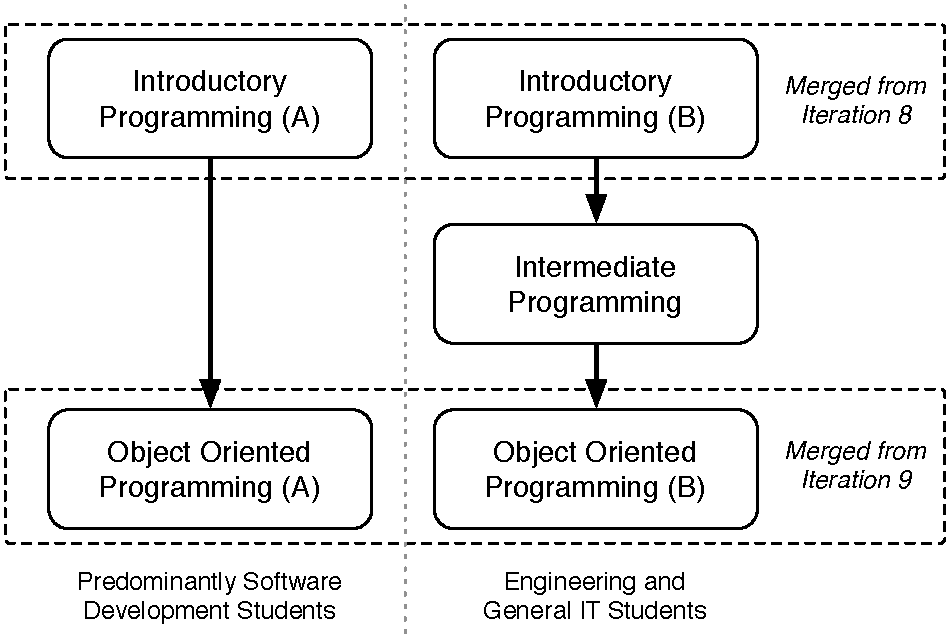
\includegraphics[width=0.8\textwidth]{UnitPaths}
  \caption{Progression pathways through the introductory programming units.}
  \label{fig:unit_paths}
\end{figure}

% subsubsection relationship_between_units (end)
% subsection the_units (end)


% cohort
% grade distributions
% student evaluations
% portfolio contents - by grade
% use of SwinGame
% general themes from portfolios
% depth of approach to learning

\subsection{Early Iterations} % (fold)
\label{sub:early_iterations}

\subsubsection{Iteration 1} % (fold)
\label{sub:iteration_1}

\paragraph{Focus} % (fold)

This was our first attempt at portfolio assessment, and so the focus for the first iteration was on implementing portfolio assessment in general. Most of our attention was on implementing changes in line with constructivist learning theories, \pref{itm:construct} from \cref{cha:guiding_principles}.

\paragraph{Action Plan} % (fold)

The approach used was an iterative step toward the general model presented in \cref{cha:approach}. Students were required to complete six assignments and six tests, with the \emph{option} to include a portfolio. The aim of the assessment strategy was for students to demonstrate their understanding of core concepts in the assignments and tests, with the portfolio used to determine student ability in the higher grade brackets. Appropriate weights were applied to each of the assessment items and these were added together to calculate the final grade.

Key differences from the portfolio model presented in \cref{cha:approach}:
\begin{itemize}[noitemsep,nolistsep]
  \item The unit included a total of eleven intended learning outcomes, each making use of active verbs and relating to specific parts of the unit.
  \item It used multiple assignments (six) over the semester.
  \item It included tests that were marked and contributed to the final grade.
  \item Submission of a portfolio was optional.  All students who submitted a portfolio were interviewed.
\end{itemize}

Similarities with later portfolio iterations included:
\begin{itemize}[noitemsep,nolistsep]
  \item It included criteria for each grade, though these were described in general terms.
  \item Students included a self assessment against the criteria.
\end{itemize}

Key differences from the introductory programming unit described in \cref{cha:example_impl} included the following:
\begin{itemize}[noitemsep,nolistsep]
	\item Focus was on programming concepts, but there was more crossover of topics in the early material.
	\item The teaching and learning activities made limited use of SwinGame.
	\item Procedures were introduced later, as SwinGame was not used in the early parts of the teaching period. 
	\item Students were only briefly introduced to the C programming language at the end of the unit.
	\item None of the supporting tools from \cref{cha:supporting} had been developed at this stage.
	\item Lecture slides closely followed the ``Beyond Bullet Points'' approach \cite{Atkinson:2007}, and included extensive notes on each slide.
	\item An earlier edition of the Pascal Language Reference \cite{FPC:2013lang} was used as the unit text.
\end{itemize}

\paragraph{Data} % (fold)

Unit results across all iterations are shown in \tref{tbl:unit_results}. This lists the number of students receiving each grade over the nine iterations. Grades include those students who enrolled but did not submit a portfolio (NA) those who failed (N) and those who received Pass (P) Credit (C) Distinction (D) and High Distinction (HD) result. The results for Iteration 1 are shown in \fref{fig:iterations_1_2}. In this iteration a large percentage of students managed to receive an HD grade.

\begin{table}[htbp]
  \footnotesize
  \renewcommand{\arraystretch}{1.3}
  \caption{Unit Results Across Iterations 1 to 9 for the introductory programming and object oriented programming units.}
  \label{tbl:unit_results}
  \centering
    \begin{tabular}{l|l|c|c|c|c|c|c}
        Iter. & Unit    & NA & N  & P  & C  & D  & HD \\ \hline
        1         & Introductory Programming (A)  & 3  & 1  & 4  & 5  & 6  & 11 \\ \hline
        2         & Object Oriented Programming (A) & 19 & 7  & 14 & 19 & 13 & 11 \\ \hline
        3         & Introductory Programming (A)  & 9  & 1  & 2  & 9  & 6  & 9  \\ \hline
        4         & Object Oriented Programming (A) & 4  & 7  & 3  & 17 & 6  & 5  \\ \hline
        5         & Introductory Programming (A)  & 10 & 6  & 9  & 19 & 12 & 14 \\ \hline
        6         & Introductory Programming (A)  & 14 & 3  & 28 & 20 & 14 & 5  \\ \hline
        7         & Introductory Programming (B)  & 42 & 12 & 56 & 47 & 22 & 7  \\ 
        ~         & Object Oriented Programming (A) & 5  & 8  & 18 & 10 & 8  & 9  \\ \hline
        8         & Introductory Programming (A)  & 11 & 5  & 20 & 21 & 17 & 14 \\ 
        ~         & Introductory Programming (B)  & 39 & 47 & 84 & 36 & 20 & 9  \\ \hline
        9         & Introductory Programming (B)  & 61 & 4  & 78 & 24 & 25 & 7  \\ 
        ~         & Object Oriented Programming (A) & 14 & 0  & 25 & 6  & 14 & 7  \\ 
        ~         & Object Oriented Programming (B) & 7  & 0  & 25 & 5  & 3  & 4  
    \end{tabular}
\end{table}

\begin{figure}[htbp]
  \centering
  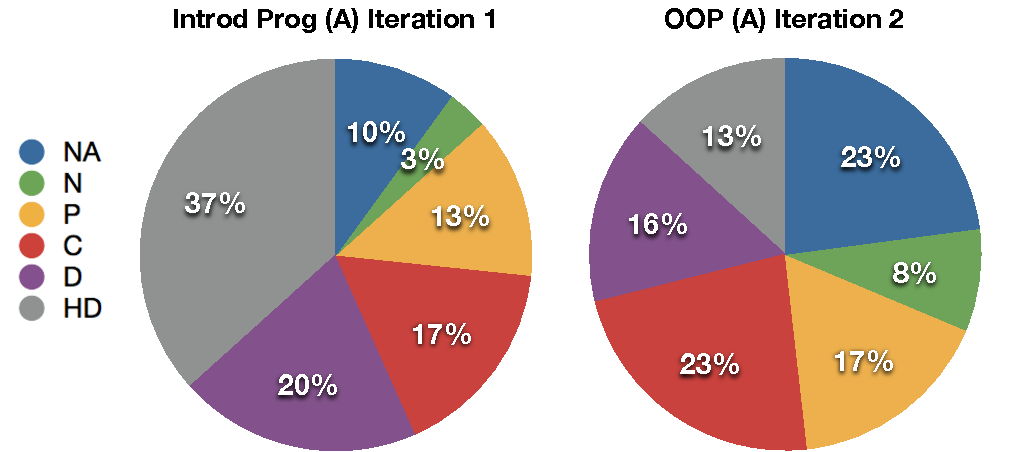
\includegraphics[width=0.8\columnwidth]{Iterations1_2}
  \caption{Result distributions from Iterations 1 and 2.}
  \label{fig:iterations_1_2}
\end{figure}

\paragraph{Reflections and Analysis} % (fold)
\label{ssub:analysis}

Staff reflections included several interesting aspects related to the assessment in this iteration:
\begin{itemize}[noitemsep,nolistsep]
  \item There were too many intended learning outcomes. This had made it difficult for staff to clearly communicate how teaching and learning activities related to the outcomes. Students had also found it difficult to relate their portfolio pieces back to the intended learning outcomes.
  \item Criteria were difficult to apply, being weakly defined, and students tended to weaken the criteria further in their self assessment.
  \item Significant effort had been put into creating ``Beyond Bullet Point'' slides and associated notes, which had been useful in terms of delivery but were restricting opportunities to adapt the material.
  \item Assessing the portfolios was very time consuming.
  \item Staff felt confident that a portfolio of work would provide a suitable means of assessing student outcomes in technical units.
  \item Core assignments and tests:
  \begin{itemize}[noitemsep,nolistsep]
    \item Covered the minimum expectations for the intended learning outcomes.
    \item Received high marks, which only indicated basic coverage of the intended learning outcomes. 
  \end{itemize}
  \item Students with weak portfolios were still able to received high grades.
\end{itemize}

Use of portfolios was limited in this iteration, with positive and negative results. The two main issues were the weakness of the expressed assessment criteria and the combining of results from the assignments and tests. Together, these issues resulted in many students receiving a higher grade than staff felt was appropriate given the outcomes demonstrated in student portfolios. This is supported by the high portion of students with HD grades.

Positive aspects of the unit delivery included the improved confidence of staff in the potential for using portfolio assessment in units related to software development. Overall, it was felt that portfolio assessment offered great potential, but that this iteration had not managed to create a suitable environment in which these benefits could be realised.

\paragraph{Development of Principles} % (fold)

The first experience of delivering a portfolio assessed unit had been informed by examining the principles of constructive alignment, and the experience provided a number of insights that helped form the principles from \cref{cha:guiding_principles}. These included:

\begin{itemize}[noitemsep,nolistsep]
	\item Constructive learning theories, \pref{itm:construct}, and aligned curriculum, \pref{itm:align}, had been at the centre of this experience. The utility of both had been hampered by the large number of intended learning outcomes. This guided the importance of having a small number of more highly targeted outcomes.
	\item The portfolios had been able to capture student outcomes, but results had been impacted by the use of grades to encourage during the semester. While alternative schemes could have been developed, it was felt these incentives were not required and a greater use of formative feedback would have benefited the students. This emphasis on formative feedback evolved into \pref{itm:formative} and influenced a change from a soft Theory X to Theory Y, \pref{itm:theory_y}.
	\item Teaching staff were \emph{willing to change}, and wanted to be able to adjust teaching material in response to student issues. However, the significant effort that had gone into the develop of the ``Beyond Bullet Points'' lecture slides provided unproductive resistance to change. This conflict started a change in attitude that resulted in the definition of \pref{itm:agile}, the aim to be both \emph{agile} and \emph{willing to change}.
\end{itemize}

% paragraph development_of_principles (end)

% subsection iteration_1 (end)

\subsubsection{Iteration 2} % (fold)
\label{sub:iteration_2}

\paragraph{Focus} % (fold)

Iteration 2 included the delivery of Object Oriented Programming (A), and aimed to address several of the main concerns from Iteration 1: having \emph{fewer ILOs} around which everything would be based, assessing each student's outcomes as a whole with \emph{100\% portfolio assessment}, and \emph{specific assessment criteria} expressing what was expected for each grade. In addition to this, the unit material was separated into teaching and learning activities and teaching and learning resources, in an effort to enable greater flexibility with future changes.

\paragraph{Action Plan} % (fold)
\label{ssub:develop_an_action_plan2}

In this iteration the following aspects of our model were included:
\begin{itemize}[noitemsep,nolistsep]
  \item We adjusted the unit to use five intended learning outcomes.
  \item Assessment criteria were developed for each grade using the different levels from the SOLO taxonomy \cite{Biggs:1982}. This was presented in a format similar to that shown in \fref{fig:assessment_criteria}, though some details differed.
  \item Feedback was provided using weekly formative assessments, and tests.
  \item Notes previously embedded in slides were shifted to a single document and distributed to students as a PDF.
\end{itemize}

The following aspects differed:
\begin{itemize}[noitemsep,nolistsep]
  \item Each intended learning outcome had criteria for meeting it to differing standards: Marginal, Adequate, Good, and Excellent.
  \item A Credit grade required three intended learning outcomes to be addressed at an \emph{Adequate} standard, Distinction required two at a \emph{Good} standard (with all other adequate) and High Distinction required two \emph{Excellent} and all others \emph{Good}.
  \item A flipped classroom model \cite{Baker:2000,Lage:2000} was adopted: student were provided with online videos covering the weekly lecture material and class room activities were predominantly interactive.
\end{itemize}

Key differences from the object oriented programming unit described in \cref{cha:example_impl} included the following:
\begin{itemize}[noitemsep,nolistsep]
	\item A greater emphasis was placed on constructive learning theories, and a shift toward discovery learning. Concepts were presented using the video podcasts, and lecture activities included a greater emphasis on group discussions.
	\item Lectures used a number of interactive quizzes, questions were typically taken then discussed in groups and retaken to see changes in understanding.
	\item Laboratory exercises also had less guidance, and students explored their chosen language and how it could be used to implement object oriented programs.
	\item While multiple languages were used, and students could only choose between the Java and C\# programming languages.
	\item SwinGame was introduced early on to enable students to visualise object interactions through the creation of a drawing program.
\end{itemize}

% subsubsection develop_an_action_plan (end)

\paragraph{Data} % (fold)
\label{ssub:data2}

\fref{fig:iterations_1_2} shows the result distributions for Object Oriented Programming (A) in Iteration 2. The number of High Distinction results was closer to expectations, though the pass rate was a cause for concern. 

\paragraph{Reflections and Analysis} % (fold)
\label{ssub:staff_reflections_and_analysis2}

Key staff reflections included:
\begin{itemize}[noitemsep,nolistsep]
  \item Interviewing all students meant that portfolio assessment was very time consuming.
  \item The general structure of the assessment criteria was suitable, but there was a disconnect in perceived standard: the interpretation of ``good'' was significantly different between staff and students.
  \item Work was of a weaker standard than desired across all grades.
  \item Students did not benefit from the classroom flip, with few preparing adequately for the classroom discussions.
  \item It was felt that many students ``coasted'' along, and did not genuinely attempt the planned activities.
  \item Progress on understanding weekly topics was very slow, with the lack of guidance resulting in students not making the best use of their time.
  \item Separation of teaching and learning activities and resources had enabled a greater freedom in creating the interactive lecture, and the resources could be reused for future unit deliveries.
\end{itemize}

Staff felt that most of the issues from the semester could be attributed to the shift toward non-productive ``discover learning'' \cite{Anderson:1998}. In our effort to implement constructive learning theories we had reduced the amount of guided learning activities, and student productivity appeared to have been adversely affected.

It was still felt that portfolio assessment could be beneficial but that, again, we had failed to realise any benefits. In many ways, the results, in terms of student learning outcomes, from this teaching period had felt like a backward step.

\paragraph{Development of Principles} % (fold)

The teaching and learning environment created in Iteration 2 had been informed by the constructive learning theories, and a trusting Theory Y environment. At the end of this iteration it was felt that the Theory Y attitude was still appropriate, but that the overly zealous application of constructive learning theories had meant students were unable to appropriately apply themselves. The lack of guidance had resulted in many students spending too much time working out what it was they needed to learn, and not enough time applying the concepts related to object oriented programming.

This experience influenced a number of the principles from \cref{cha:guiding_principles}. 

\begin{itemize}[noitemsep,nolistsep]
	\item Constructive learning theories, central to \pref{itm:construct}, were tempered to include stronger guidance along with the focus on the central role of the learning in constructing their own knowledge. 
	\item We needed to more clearly communicate our high expectations of students, which became \pref{itm:expectations}. In this iteration many students did not seem to be aware of what had been expected of them.
	\item Students had been able to reflect in their learning summary reports, \pref{itm:reflect}, but without clearly understanding the high expectations these had been shallow.
	\item The shallow responses of students also indicated the need to focus on depth of understanding, \pref{itm:depth}.
\end{itemize}

% subsection iteration_2 (end)

% subsection early_iterations (end)

\subsection{As the Model Stabilised} % (fold)
\label{sub:as_the_model_stabilised}

% subsection as_the_model_stabilised (end)

\subsection{Latest Iterations} % (fold)
\label{sub:latest_iterations}

% subsection latest_iterations (end)

% section lessions_learnt_from_action_research (end)


\section{Issues Identified in Student Reflections} % (fold)
\label{sec:issues_identified_in_student_reflections}

To ensure that all issues were reported in the results, the process we followed did not remove or ignore any issues raised. All issues that could not be grouped into an existing theme were collected together as a miscellaneous ``other'' theme. The Results section outlines the different themes identified, and how these themes relate to the comments raised by students in their reflections.

% section issues_identified_in_student_reflections (end)

\section{Evaluating Progress using Burndown Charts} % (fold)
\label{sec:evaluating_progress_using_burndown_charts}

% section evaluating_progress_using_burndown_charts (end)




% chapter lessons_learnt_through_action_research (end)